
% History and Goals Slide
\section{History and Goals}
\begin{frame}{History and Goals}
  \begin{itemize}
    \item The project started in 2006 to inspire children and improve their computing skills.
    \item It was inspired by the BBC Micro project from 1981.
    \item The official launch was on February 29, 2012, with 10,000 boards in the first run.
    \item By 2024, over 60 million units had been sold, primarily manufactured in Wales.
    \item It is the third-best-selling general-purpose computer, after the PC and the Mac.
  \end{itemize}
\end{frame}

% Raspberry Pi Products Evolution Slide

\begin{frame}{The Raspberry Pi Products Evolution}
  \begin{itemize}
    \item Raspberry Pi 1 Model B
    \item Raspberry Pi 2/3 Model B/B+
    \item Raspberry Pi 4 Model B
    \item Raspberry Pi Zero
    \item Raspberry Pi Compute Module
    \item Raspberry Pi 5 Model B
  \end{itemize}
  \begin{center}
    \includegraphics[width=0.8\textwidth]{trainingmaterials/rpibasics/evolution.png} 
  \end{center}
\end{frame}

% Block Diagram Slide
\begin{frame}{Block Diagram}
  \begin{center}
    \includegraphics[width=0.8\textwidth]{trainingmaterials/rpibasics/rpiblockdiagram.png} % Replace with the actual image file
  \end{center}
\end{frame}

% Hardware Specifications Slide
\section{Hardware Specifications}
\begin{frame}{Hardware Specifications I}
  \begin{itemize}
  \item \textbf{Broadcom SoC:} Includes CPU, GPU, and DSP.
      \begin{itemize}
        \item RPI1: BCM2835, ARM 11 at 700MHz (ARMv6)
        \item RPI2: BCM2836, Quad-Core ARM Cortex A7 at 900MHz (ARMv7-A)
        \item RPI3: BCM2837, Quad-Core ARM Cortex A53 at 1.2GHz (ARMv8)
        \item RPI4: BCM2711, Quad-Core ARM Cortex A72 at 1.5GHz (ARMv8)
        \item RPI5: BCM2712, Quad-Core ARM Cortex A76 at 2.4GHz (ARMv8)
      \end{itemize}   
  \item \textbf{Memory:} The RAM is physically stacked on top of the Broadcom media processor (package-on-package technology). Ranges from 512MB (RPI1) to 8GB (RPI5).
  \item \textbf{GPU: }Provides OpenGL ES 1.1, OpenGL ES 2.0, hardware-accelerated OpenVG 1.1, Open EGL, OpenMAX and 1080p30 H.264 high-profile decode. Increase in clock frequency and 3D capabilities with the new models.
   \end{itemize}
\end{frame}

\begin{frame}{Hardware specifications II}
    \begin{itemize}
        \item LAN9512 providing: 10/100Mb Ethernet (Auto-MDIX) (RPI4 and RPI5 supports 1GbE)
        \item 2x USB 2.0 (RPI), 4 xUSB 2.0 in (RPI2/3), 2 xUSB 2.0 + 2 xUSB 3.0 (RPI4 and RPI5)
        \item Power: 5V DC (RPI 1-3 via micro-USB, RPI4/5 via USB-C)
        \item DSIinterface. 15-pin surface mounted flat flex connector, providing two data lanes, one clock lane, 3.3V and GND.
        \item HDMI connector providing type with A HDMI 1.3a out (RPI4/5 2x micro-HDMI)
    \end{itemize}
\end{frame}

\begin{frame}{Hardware specifications III}
\begin{itemize}
    \item Composite Video connector: RCA (RPI1)
     \item MIPICSI-2interface. 15-pin surface mounted flat flex connector.
     \item Audio connector: 3.5mm stereo jack (output only)
     \item SD/MMC/SDIO memory card slot (underside) (microSD since RPI2)
     \item 40-pin (2x20) 2.54 mm header expansion, providing: (26 on RPI1):
         \begin{itemize}
             \item 12 GPIOsat 3v3
            \item 2-pin UART serial console, 3v3 TTL (debug); or 2 GPIOs at 3v3
            \item I²C interface (3v3); or 2 GPIOs at 3v3
            \item SPI interface (3v3); or 5 GPIOs at 3v3
            \item 3v3, 5v and GND supply pins
            \item ARM JTAG (if pins are reconfigured in software - on Revision1.0 boards one signal would also need to be taken from S5)
            \item I²S interface (if pins are reconfigured in software, hardware hack may be required)
         \end{itemize}
\end{itemize}
\end{frame}

\begin{frame}{Hardware specifications IV}
    \includegraphics[scale=0.8]{trainingmaterials/rpibasics/RPIand40pin.pdf}
\end{frame}
% First Software Steps Slide
\section{First Software Steps}
\begin{frame}{First Software Steps with RPI}
  \begin{itemize}
    \item \textbf{Operating Systems:}
    \begin{itemize}
      \item Raspbian: Debian-based distribution.Linux Debian-based distribution created by Raspberry-PI organization Installation process documented in Raspberry-PI foundation website You don’t need a hard disk but an SD-Card (as faster as possible). Complete Linux with development toots and applications
      \item Ubuntu Core: Designed for IoT applications.
    \end{itemize}
    \item \textbf{Bare metal}
    \item \textbf{Software Tools:}
    \begin{itemize}
      \item GNU Compiler, linker, and debuggers for ARM processors.
      \item Programming in C and C++.
      \item Command line or Eclipse GUI.
    \end{itemize}
  \end{itemize}
\end{frame}



% Embedded Systems Slide
\section{Embedded Systems}
\begin{frame}{What are Embedded Systems?}
  \begin{columns}
      \begin{column}{0.5\textwidth}   
          \begin{itemize}
            \item Specialized computing system with specific-purpose hardware and software.
            \item Part of a larger system with real-time constraints.
            \item Examples: Router, network switch, smartphones, smartwatches, printers, gaming consoles.
          \end{itemize}
      \end{column}
  \begin{column}{0.5\textwidth} 
  \begin{center}
    \includegraphics[width=0.8\textwidth]{trainingmaterials/rpibasics/embeddedsystem.png} 
  \end{center}
  \end{column}
 \end{columns}
\end{frame}

\begin{frame}{What ``embedded'' can mean}
\begin{itemize}
  \item \textbf{Ultra-low power control:} coin-cell sensors, simple I/O
  \item \textbf{Connected IoT:} Wi-Fi/BLE + cloud, security updates
  \item \textbf{Real-time control:} motor control, deterministic timing
  \item \textbf{Compute-heavy edge:} vision/AI, multimedia, gateways
  \item \textbf{Hardware-accelerated edge:} high-speed I/O, low-latency pipelines
  \item \centering 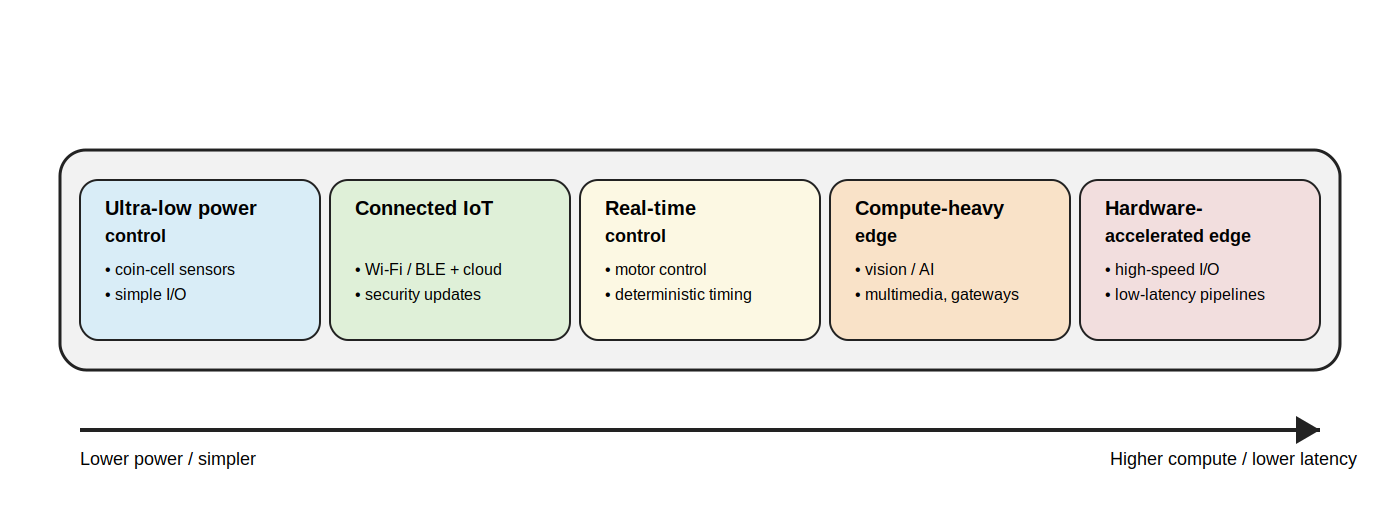
\includegraphics[width=12cm]{trainingmaterials/rpibasics/use_case_spectrum.jpg}
\end{itemize}
\end{frame}


\begin{frame}{Key decision criteria}
\begin{itemize}
  \item \textbf{Real-time needs:} hard/soft deadlines, jitter tolerance
  \item \textbf{Power budget:} sleep current, duty cycle, battery life
  \item \textbf{Connectivity:} BLE/Wi-Fi/Ethernet/Cellular, certifications
  \item \textbf{Cost \& BOM:} unit cost, availability, supply chain risk
  \item \textbf{Security \& updates:} secure boot, OTA, long-term patching
  \item \textbf{Time-to-market:} dev tools, ecosystem, reference designs
  \item \textbf{Throughput/latency:} sensor rates, DMA, bandwidth, deterministic pipelines
\end{itemize}
\end{frame}

\begin{frame}{Alternative \#1: Bare-metal microcontroller (MCU)}
\textbf{What it is:} Firmware directly on MCU, no OS
\vspace{0.6em}

\textbf{Pros}
\begin{itemize}
  \item Lowest cost/power, fast boot
  \item Simple stack, predictable behavior
\end{itemize}

\textbf{Cons}
\begin{itemize}
  \item Complexity grows fast (timers, comms, features)
  \item Harder to maintain at scale
\end{itemize}

\textbf{Use when:} simple control logic, strict power, minimal features.
\end{frame}


\begin{frame}{Alternative \#2: MCU + RTOS}
\textbf{RTOS options often considered:}
\begin{itemize}
  \item FreeRTOS
  \item Zephyr
  \item ThreadX / Azure RTOS
  \item CMSIS-RTOS V2 API
\end{itemize}

\textbf{Pros}
\begin{itemize}
  \item Better structure (tasks, queues), real-time scheduling
  \item Scales to moderate complexity
\end{itemize}

\textbf{Cons}
\begin{itemize}
  \item More learning curve, debugging concurrency
  \item Still resource-constrained vs Linux
\end{itemize}
\end{frame}


\begin{frame}{Alternative \#3: Embedded Linux on MPU/SoC}
\textbf{What it is:} Linux on a microprocessor/SoC (often ARM)
\vspace{0.6em}

\textbf{Pros}
\begin{itemize}
  \item Rich networking, security tooling, filesystems, containers
  \item Faster feature development (Python, Go, etc.)
\end{itemize}

\textbf{Cons}
\begin{itemize}
  \item More power, slower boot
  \item More complexity (kernel, drivers, build systems)
\end{itemize}

\textbf{Use when:} User Interface, gateways, networking, complex updates.
\end{frame}


\begin{frame}{Alternative \#4: Single-Board Computer (SBC)}
\textbf{Mindset:} ``ready-to-run Linux board''
\vspace{0.6em}

\textbf{Pros}
\begin{itemize}
  \item Fast prototyping, lots of I/O and community support
  \item Lower Non-Recurrent Engineering (NRE)initially
\end{itemize}

\textbf{Cons}
\begin{itemize}
  \item Not always product-friendly (size, connectors, lifecycle)
  \item Supply chain variability
\end{itemize}

\textbf{Common for:} prototypes, pilots, internal tools.
\end{frame}


\begin{frame}{Alternative \#5: System-on-Module (SoM) + custom carrier}
\textbf{What it is:} compute module + your custom carrier board
\vspace{0.6em}

\textbf{Pros}
\begin{itemize}
  \item Speeds hardware design while keeping product-ready custom I/O
  \item Better path to certification and manufacturing than SBC
\end{itemize}

\textbf{Cons}
\begin{itemize}
  \item More engineering than SBC
  \item Vendor lock-in considerations
\end{itemize}
\end{frame}


\begin{frame}{Alternative \#6: SoC/SiP(System in Package) direct-to-board (full custom)}
\textbf{What it is:} place the SoC + DDR + Power management yourself
\vspace{0.6em}

\textbf{Pros}
\begin{itemize}
  \item Lowest unit cost at scale, full control of design
\end{itemize}

\textbf{Cons}
\begin{itemize}
  \item Highest NRE, hardest layout (DDR), more risk/time
\end{itemize}

\textbf{Use when:} high volume + strong hardware team + stable requirements.
\end{frame}


\begin{frame}{Alternative \#7: FPGA (programmable logic)}
\textbf{What it is:} Configurable hardware fabric for custom datapaths and I/O.
\vspace{0.6em}

\textbf{Pros}
\begin{itemize}
  \item Deterministic latency, true parallelism, custom interfaces
  \item Great for high-speed acquisition (ADC/DAC), framing, filtering, pre-processing
\end{itemize}

\textbf{Cons}
\begin{itemize}
  \item Tooling and verification complexity
  \item Power/cost can rise if over-provisioned
\end{itemize}

\textbf{Use when:} strict latency/throughput, unusual I/O, streaming pipelines.
\end{frame}


\begin{frame}{Alternative \#8: SoC-FPGA (CPU + FPGA on one chip)}
\textbf{What it is:} Hardened CPU (often ARM) + FPGA fabric + shared memory/DMA.
\vspace{0.6em}

\textbf{Pros}
\begin{itemize}
  \item Best of both: Linux/RTOS control plane + FPGA data plane
  \item Tight integration (low-latency DMA), fewer chips/boards
\end{itemize}

\textbf{Cons}
\begin{itemize}
  \item Complex partitioning (what runs where) and bring-up
  \item Vendor ecosystems / toolchains
\end{itemize}

\textbf{Use when:} you need software flexibility + hardware acceleration in one device.
\end{frame}


\begin{frame}{Alternative \#9: ACAP (adaptive compute acceleration platform)}
\textbf{What it is:} heterogeneous compute (programmable logic + DSP/AI engines + CPUs)
designed for acceleration workloads.
\vspace{0.6em}

\textbf{Pros}
\begin{itemize}
  \item Mix-and-match engines for \textbf{throughput} and \textbf{low latency}
  \item Better fit for complex pipelines (signal processing, AI inference, networking)
\end{itemize}

\textbf{Cons}
\begin{itemize}
  \item Platform maturity, toolchain learning curve
  \item Overkill for simple embedded control
\end{itemize}

\textbf{Use when:} you need multiple accelerators and sustained high performance at the edge.
\end{frame}


% % ---------------- Updated decision flow slide ----------------
% \begin{frame}{OS/Platform decision flow (simple)}
% \begin{columns}[T,onlytextwidth]
%   \begin{column}{0.55\textwidth}
%     \begin{enumerate}
%       \item \textbf{Need Linux apps/UI/containers?} $\rightarrow$ Linux (SBC or SoM)
%       \item Else \textbf{hard real-time / many concurrent features?} $\rightarrow$ MCU + RTOS
%       \item Else \textbf{simple + ultra-low power + low cost?} $\rightarrow$ Bare metal MCU
%       \item \textbf{Need strict throughput/latency or custom I/O?} $\rightarrow$ FPGA / SoC-FPGA / ACAP
%     \end{enumerate}
%   \end{column}
%   \begin{column}{0.45\textwidth}
%     \centering
%     \includesvg[width=\linewidth]{figures/decision_flow_fpga_acap}
%     \vspace{0.3em}
%     {\scriptsize Includes acceleration path.}
%   \end{column}
% \end{columns}
% \end{frame}

% % ---------------- Slide: Where acceleration fits ----------------
% \begin{frame}{Where FPGA/SoC-FPGA/ACAP fit (data plane vs control plane)}
% \centering
% \includesvg[width=0.92\linewidth]{figures/control_data_plane_fpga_acap}
% \vspace{0.4em}

% {\scriptsize Typical split: CPU runs orchestration; fabric/engines run the high-rate pipeline.}
% \end{frame}

% % ---------------- Slide  (architecture patterns updated) ----------------
% \begin{frame}{Architecture patterns (how you build it)}
% \begin{columns}[T,onlytextwidth]
%   \begin{column}{0.55\textwidth}
%     \begin{itemize}
%       \item \textbf{Monolith firmware} (small MCU projects)
%       \item \textbf{Layered HAL + drivers + services} (scales better)
%       \item \textbf{RTOS tasks + message queues} (modular + testable)
%       \item \textbf{Linux: services + IPC + OTA pipeline} (maintainable fleets)
%       \item \textbf{CPU control plane + accelerated data plane} (FPGA/ACAP designs)
%     \end{itemize}
%   \end{column}
%   \begin{column}{0.45\textwidth}
%     \centering
%     \includesvg[width=\linewidth]{figures/architecture_patterns_fpga_acap}
%     \vspace{0.3em}
%     {\scriptsize Adds accelerated pipeline pattern.}
%   \end{column}
% \end{columns}
% \end{frame}

% % ---------------- Slide ----------------
% \begin{frame}{Risk checklist (what bites later)}
% \begin{itemize}
%   \item Component lifecycle \& second sources
%   \item OTA strategy and secure boot
%   \item Regulatory/certification for radio
%   \item Debug/telemetry in the field
%   \item Production test strategy (fixtures, flashing, calibration)
%   \item \textbf{FPGA/ACAP-specific:} verification, timing closure, bitstream security, field updates
% \end{itemize}
% \end{frame}


% Design Constraints Slide





% Embedded System Design with Raspberry Pi Slide
\section{Designing with Raspberry Pi}
\begin{frame}{Embedded System Design with Raspberry Pi}
  \begin{itemize}
    \item Use an ARM multicore platform
    \item Use of embedded peripherals
    \item Sensor interface using I2C
    \item Use of Embedded Linux as Operating System
    \item Develop applications in C/C++ with the help of Linux Kernel functionalities
    \item Develop, debug, and deploy applications using:
    \begin{itemize}
        \item GNU tools
        \item Eclipse Environment and/or Visual Code
    \end{itemize}
\end{itemize}
\end{frame}

% Market Trends Slide

\section{Market Trends}
\begin{frame}{Market Trends I}
  \begin{itemize}
    \item \centering \includegraphics[scale=0.5]{trainingmaterials/rpibasics/torizon-hw.png}.
    \item \includegraphics[scale=0.5]{trainingmaterials/rpibasics/Montavista.png}
  \end{itemize}
\end{frame}


\begin{frame}{Market Trends II}
    \begin{itemize}
        \item Industrial grade Linux
        \item Powerful features to build state-of-the-art embedded solutions
        \item Strong focus on Security with container support and services
        \item Time-saving and cost-efficient application development
        \item Drivers, connectivity stacks, real-time extensions, support for industrial hardware and graphical development environment
        \item Engineers support with experience in industrial applications
    \end{itemize}
    \begin{itemize}
        \item \centering \includegraphics[scale=0.15]{trainingmaterials/rpibasics/SYSGO_graphic_elinos_embedded_linux.png}
    \end{itemize}
\end{frame}


\begin{frame}{Market Trends in Advanced Embedded Systems}
  \begin{itemize}
    \item Increasing adoption of AI engines and DSP engines.
    \item Use of adaptable hardware (e.g., Xilinx Versal, Intel Agilex).
    \item Embedded Linux plays a critical role in modern systems.
    \begin{itemize}
        \item \centering \includegraphics[scale=0.5]{trainingmaterials/rpibasics/xilinxacap.png}
    \end{itemize}
  \end{itemize}
\end{frame}

% Student Research Slide
\section{Student Research}
\begin{frame}{Student Research Topics I}
 Research about these questions and prepare a report (you have to submit it to moodle)
 \begin{itemize}
    \item What is the architecture of the Raspberry Pi 4 Model B+ core? Is it a 32-bit or 64-bit core?
    \item What is bare-metal programming?
    \item What software tools are required for bare-metal programming?
    \item What are the advantages/disadvantages of using bare metal programming vs. operating system programming?
    \item What are the typical compilers and linkers used in Linux OS?
    \item Review the concepts of compile and link. Could you explain the difference among a compile, link and execution error? Give an example.
    \item What is a library? What extensions do the libraries files have?
    \item What is the purpose of the Linux “make” command?
    \item What is a Makefile file?
    \item What do user space and kernel space mean in Linux?
    
\end{itemize}
\end{frame}

\begin{frame}{Student Research Topics II}
 \begin{itemize}
    \item Identify the steps to compile a program in GNU/Linux using gcc and g++
    \item What is the purpose of glibc library in GNU/Linux?
    \item What is the utility to debug C/C++ applications with GNU tools? 
    \item What is a GPU?
    \item What are the main advantages of using GPUs?
    \item What is the typical programming method for developing applications with GPUs?
    \item Identify the most common Linux Distributions. What are the differences among them?
\end{itemize}
\end{frame}



